\documentclass[a4paper,times,12pt]{article}
%\usepackage{indentfirst}
\usepackage{amsmath}
\usepackage{multirow}
\usepackage{graphicx}
\usepackage{float}
\usepackage{setspace}
%\usepackage{svg}
\usepackage{subcaption}
%\usepackage{minted}
\onehalfspacing
\usepackage[top=2.5 cm, bottom=2.5 cm, left=4 cm, right=2.5 cm]{geometry}
%\usepackage{hyperref}
\usepackage{algorithm}
\usepackage{rotating}
\usepackage[noend]{algpseudocode}

\makeatletter
\def\BState{\State\hskip-\ALG@thistlm}
\makeatother

\newcommand\tab[1][0.5cm]{\hspace*{#1}}

\setlength\parindent{0pt}

\begin{document}

\begin{titlepage}
\begin{center}
\vspace*{1cm}
\underline{\textbf{\Large ISTANBUL TECHNICAL UNIVERSITY}} \\[10 pt]

\underline{\textbf{\large FACULTY OF SCIENCE AND LETTERS}} \\[15 pt]

\textbf{\large Graduation Project} \\
\vspace{1.8 cm}

\includegraphics[scale=1.2]{itu_logo.pdf} \\
\vspace{1.8 cm}
%\textbf{\large Machine Learning and Nonlinear Schr{\"o}dinger Equation} \\[5 pt]
\textbf{\large Machine Learning and Non-linear Schr{\"o}dinger Equation} \\[5 pt]
\textbf{H{\"u}seyin Talha \c{S}enya\c{s}a}\\
\vspace{1.5 cm}
\end{center}
\vfill
\textbf{{Department : Physics Engineering}}\\
    \textbf{Student ID \hspace{0.2 cm}: 090120132}\\
    \textbf{Advisor\hspace{1.1 cm}: Assoc. Prof. A. Levent Suba\c{s}{\i}}
\vspace{2 cm}

\center\textbf{FALL 2017}

\end{titlepage}


%\title{\textbf{TEST}}
%\date{}
%\maketitle
\setcounter{page}{1}
\pagenumbering{roman}

\section*{Summary}

We train an artificial neural network to estimate the ground state energy
of a one-dimensional Bose-Einstein condensate in harmonic trapping potential.
Such a system can be described by the solution of a non-linear Schr{\"o}dinger equation also called a Gross-Pitaevskii equation. We also use the method for the inverse problem of predicting the non-linearity parameter using the ground
state density profile for a given harmonic trapping potential.

\newpage
\tableofcontents

\newpage

\pagenumbering{arabic}
\section{Introduction and Motivation}
\label{sec:Intro}
\noindent Machine learning.\\
General usage area.\\
ML in physics and Phyiscs in ML.\\
ML\&SE article.\\
Ours difference.\\

\section{Gross Pitaevskii Equation}
\subsection{General information about GPE}
\subsection{Why and how nonlinearty is introduced.}
\subsection{Physical and mathematical interpretation of interaction parameter. (phy: attractive, repulsive  math:dominance of the terms)}
\subsection{Stationary form.}
\subsection{Potential, kinetic and interaction energy expressions.}
\subsection{Reduction of dimension.}
\subsection{Analytic solution and approximation.}

\subsection{Numeric Solution and Dataset Generation}

\subsubsection{Scaling}

The scaling of GPE is generally done according to potential type and there are more than one scaling conventions \textbf{REFS}. In our study, we use a more general scaling to investigate how different scalings affect the precision. To do that, we compare numerical solutions by representing same physical system with different scaling coefficients in both framework. Then we compare these results first internally and then we do a cross check. 

We also compare numerical solutions of two different solvers implemented in different frameworks to show that the numerical solutions are \textbf{consistent}.\\ 

GPE is given as,

\begin{equation}
    \label{eq:GPE_1D}
    \frac{-\hbar^2}{2m}\frac{d^2\psi}{dz^2} + V(z)\psi + g|\psi|^2\psi = \mu\psi
\end{equation}

First we define dimensionless potential, and then we make the length dimensionless,

$$ \overline{V}(z) \equiv \frac{V(z)}{\gamma E_0}, \qquad \widetilde{z} \equiv \frac{z}{\beta L} $$

Here $\gamma$ and $\beta$ positive real numbers. $E_0$ is in energy unit and $L$ is in length and they are defined respectively as;

$$E_0 = \frac{\hbar^2}{2m} $$


$$ \widetilde{V}(\widetilde{z}) \equiv \overline{V}(\beta L z) $$ 

If these transformations are pluged into the Eq.~\eqref{eq:GPE_1D} it becomes,

\begin{equation}
    \label{eq:GPE_1D_dimensionless_en_len}
    \frac{-\hbar^2}{2m\gamma E_0} \frac{1}{\beta^2 L^2}  \frac{d^2\psi}{d \widetilde{z}^2} + \widetilde{V}(\widetilde{z})\psi + \frac{g}{\gamma E_0}|\psi|^2\psi = \frac{\mu}{\gamma E_0}\psi
\end{equation}

To obtain final form, we define dimensionless energy, wave function and interaction parameter respectively. 

$$\widetilde{\mu} \equiv \frac{\mu}{\gamma E_0}, \qquad \widetilde{\psi} \equiv \psi{\sqrt{\frac{\beta L}{N}}}, \qquad \widetilde{g} \equiv \frac{gN}{\gamma E_0 \beta L} $$

To control scaling coefficients we set the coefficient of the kinetic term to an arbitrary positive real number $\alpha$  

$$ \alpha = \frac{\hbar^2}{2m\gamma E_0} \frac{1}{\beta^2 L^2} , $$

and set $E_0 = \hbar^2 / 2m$. Now the scaling of GPE can be controlled by $\alpha$ and $\beta$ only.

\begin{equation}
\label{eq:GPE_dimensionless}
    -\alpha\frac{d^2\widetilde{\psi}}{d\widetilde{z}^2} + \widetilde{V}(\widetilde{z})\widetilde{\psi} + \widetilde{g}|\widetilde{\psi}|^2 \widetilde{\psi} = \widetilde{\mu} \widetilde{\psi}
\end{equation}
    
We are going to change these scaling coefficients and see their effects by comparing results. An example of setting the scale coefficients is shown in appendix~\ref{ap:scale}.



\graphicspath{{"../figs/numericanalyze/"}}
\begin{figure}[H]
    \centering
    \begin{subfigure}[t]{0.45\textwidth}
		%\centering
        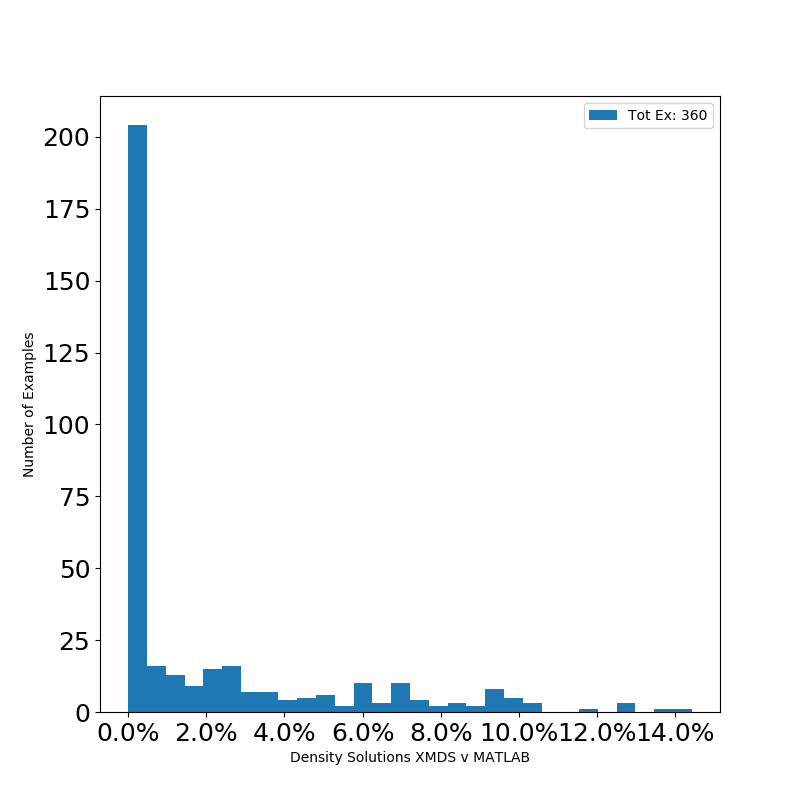
\includegraphics[width=\linewidth]{dens}
		
    \end{subfigure}
    \begin{subfigure}[t]{0.45\textwidth}
		%\centering
        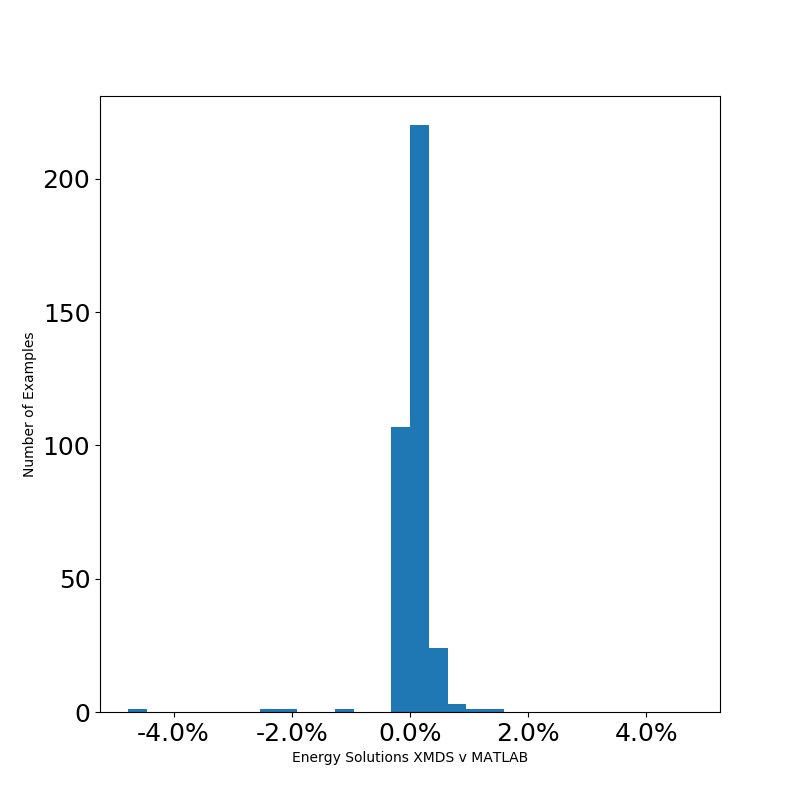
\includegraphics[width=\linewidth]{energy}
		
    \end{subfigure}
    \caption{Error in density and energy}
\label{fig:dens_energy_error}
\end{figure}


\graphicspath{{"../figs/potentials/"}}
\begin{figure}[H]
    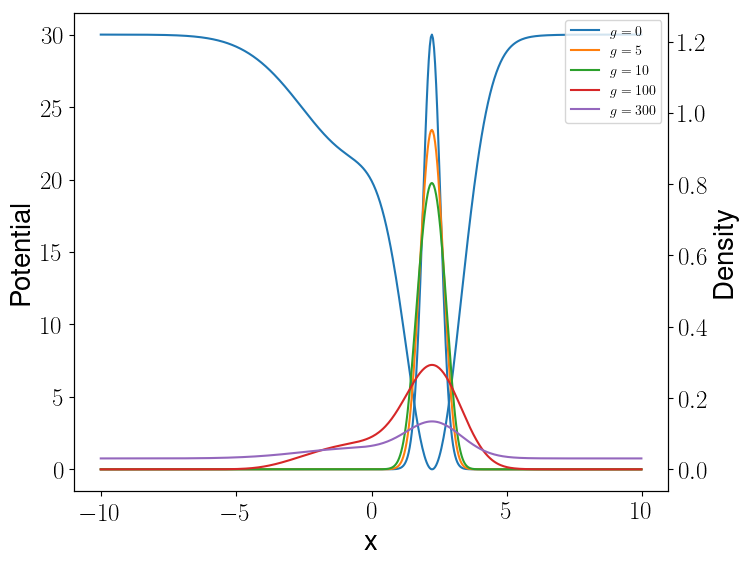
\includegraphics[width=\linewidth]{solutionswithinter}
    \caption{Density under Double Inverted Gaussian Potential with different interaction parameter.}
\label{fig:gaussian_pot_and_density}
\end{figure}

\subsubsection{Brief info about imaginary time evolution. (detailed in APPENDIX)}
\subsubsection{XMDS framerwork and other programs.}
\subsubsection{Potential generation}

In potential generation, we built a modular structure such that the algorithms to generate potentials are independent from the restrictions forced by numerical techniques such as boundary conditions or scaling. The generated potentials are sent to another method supplied by module, and this method rescales, and applies a envelope functions to ensure that potential goes to numerical limit at boundaries.

The envelope functions is defined as,
\begin{equation}
\label{eq:envelope_potential}
    \text{env}(x) = \tanh{(\beta(x + x_l))} + \tanh{(\beta(x + x_r))}
\end{equation}

where $x_l$ and $x_r$ bounds are given in the Table~\ref{tb:general_table} and the plot is given in Fig.~\ref{fig:envelope_and_random_withot_pros}. As it is shown, envelope function goes to zero at values greater than $x_r$ or lower than $x_l$ and the rapidness is proportional with $\beta$.

\graphicspath{{"../figs/potentials/"}}
\begin{figure}[H]
\centering
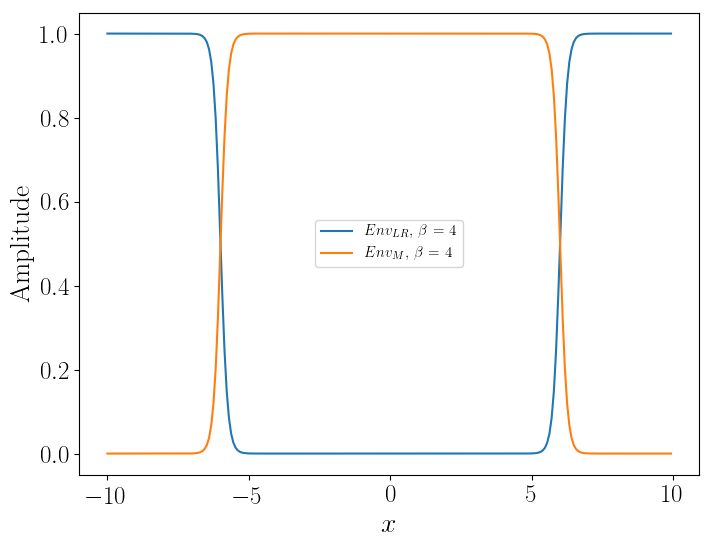
\includegraphics[width=\linewidth]{env}
\caption{Envelope Function}
\label{fig:envelope_and_random_withot_pros}
\end{figure}

The two potential in Figure~\ref{fig:envelope_and_random_withot_pros} are combined and a gaussian filter applied. 

\graphicspath{{"../figs/numericanalyze/"}}
\begin{figure}[H]
\centering
\begin{subfigure}[t]{0.45\textwidth}
    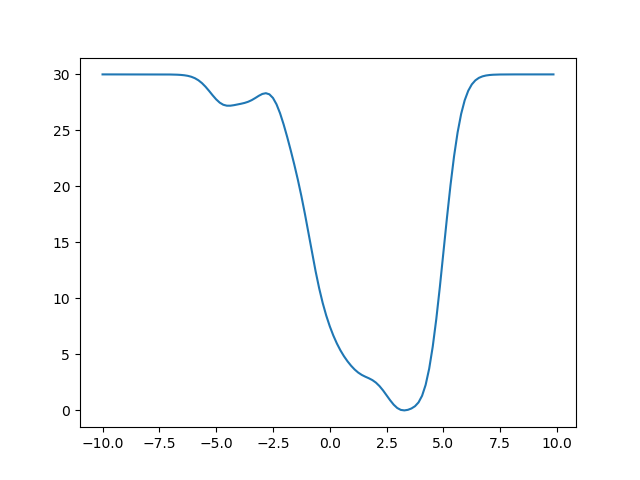
\includegraphics[width=0.5\linewidth]{rndpot}
\end{subfigure}
\centering
\begin{subfigure}[t]{0.45\textwidth}
    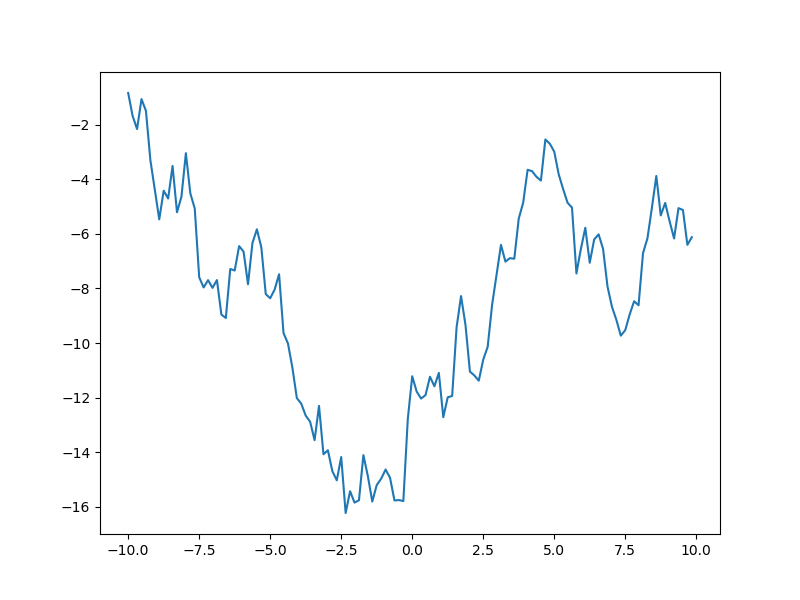
\includegraphics[width=\linewidth]{rndpotwithoutprocess}
\end{subfigure}
\end{figure}




\subsubsection{Potential types (with analytic forms etc.)}

We use \textbf{six} different types of potential in our study. The first three potential which have analytic form given in Table~\ref{tb:general_table}. are 1D version of potentials studied in \cite{mills2017deep}. We implement two more random potential generator to study effect of generation process. The generation processes of the random potentials are described in Section~\ref{sec:random_potential_gen}.

\newcommand{\infinitewell}{$
V(x) = 
    \begin{cases}
       0 &\quad\text{if } x_l < x < x_r  \\
       \infty &\quad\text{if } \textit{otherwise} \\
    \end{cases}
$}

\newcommand{\harmonicpot}{$ V(x) =  \frac{1}{2}m \omega^2 (x - x_0) ^2 $}

\newcommand{\gaussianpot}{$ V(x) = -A_1 \exp(\frac{(x - \mu_1)^2}{\sigma_1^2}) -A_2 \exp(\frac{(x - \mu_2)^2}{\sigma_2^2})  $
}

\newcommand{\randomexplation}{Summation of sines and cosines with random coefficients}

\begin{sidewaystable}
\begin{table}[H]
\centering
\caption{Potentials}
\label{tb:general_table}
\begin{tabular}{|l|l|l|l|l|} \hline
Potential                      & Analytic Form / Explanation         & Parameters           & Min   & Max  \\ \hline
\multirow{3}{*}{Infinite Well} & \multirow{3}{*}{\infinitewell}      & $x_l$                & -9    & 4.5  \\ 
                               &                                     & $x_r$                & -4.5  & 9    \\
                               &                                     & $x_r - x_l$          & 1     & 8    \\ \hline
\multirow{2}{*}{Harmonic}      & \multirow{2}{*}{\harmonicpot}       & $\omega$             & 0.01  & 3    \\ 
                               &                                     & $x_0$                & -5    & 5    \\ \hline
\multirow{3}{*}{DI Gaussian}   & \multirow{3}{*}{\gaussianpot}       & $A_1, A_2$           & 1     & 10   \\ 
                               &                                     & $\mu_1, \mu_2$       & -5    & 5    \\
                               &                                     & $\sigma_1, \sigma_2$ & 0.5   & 4    \\ \hline
Random1                        & Random walk with random step size   & Step Size (Y axis)   & -4    & 4    \\ \hline
\multirow{4}{*}{Random2}       & \multirow{4}{*}{\randomexplation}   & Number of Terms      & 1     & 100  \\ 
                               &                                     & $A_1, A_2$           & -4    & 4    \\
                               &                                     & $n_1, n_2$           & -6.30 & 6.30 \\
                               &                                     & $\sigma$             & 0.1   & 10   \\ \hline 
Random3                        & Substraction of two binary grid     & Scale Factor         & 8     & 8    \\ \hline
Random4                        &                                     &                      &       &      \\ \hline 
\end{tabular}
\end{table}
\end{sidewaystable}



\subsubsection{Random potential generations with different method. (Reason)}
\label{sec:random_potential_gen}

To be able to observe the effect of random potential generation to the results we use three different random potential generation algorithms. The first one is random walk with random step size such that the first value of the potential array is initialized with a random number. After that, another random number is added to this value to obtain the next element of the array and so on. The distribution of the random numbers is gaussian in this process. The resultant array is not guaranteed to be smooth. Gaussian filter is applied with a random sigma value to the potential array to make it smooth.    

\begin{algorithm}[H]
    \caption{RandomPotential1}\label{euclid}
    \begin{algorithmic}[1]
    \Procedure{RandomPotential1}{}
        \State $ Points = GaussianDistributedRandomPoints()$
        \State $Len = \textit{Length(Points)}$
        \State $Potential[0] = Points[0]$
        \For{$\text{i} = 0 \textbf{ to } Len - 1$}
        \State $Potential[i + 1] = Potential[i] + Points[i]$
        \EndFor
        \State $Potential = GaussianFilter(Potential, \sigma)$ 
    \EndProcedure
    \end{algorithmic}
\label{alg:random_potential_1}
\end{algorithm}

\graphicspath{{"../figs/potentials/"}}
\begin{figure}[H]
    \centering
    \begin{subfigure}[t]{0.45\textwidth}
		%\centering
        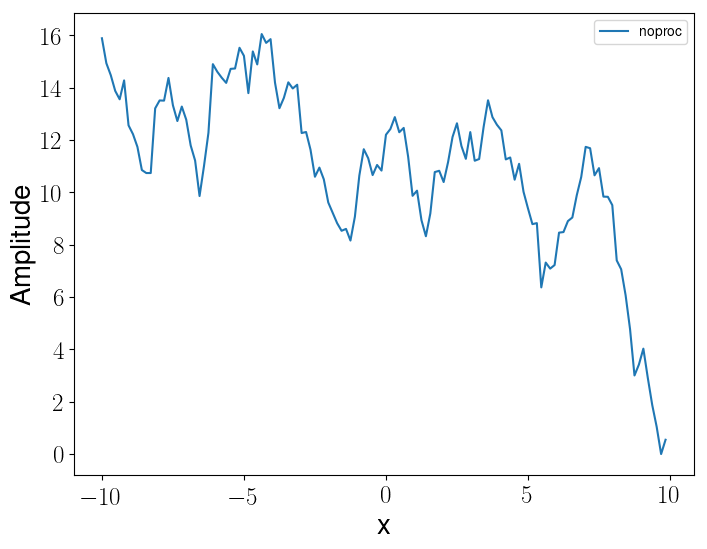
\includegraphics[width=\linewidth]{random-1-noproc}
		
    \end{subfigure}
    \begin{subfigure}[t]{0.45\textwidth}
		%\centering
        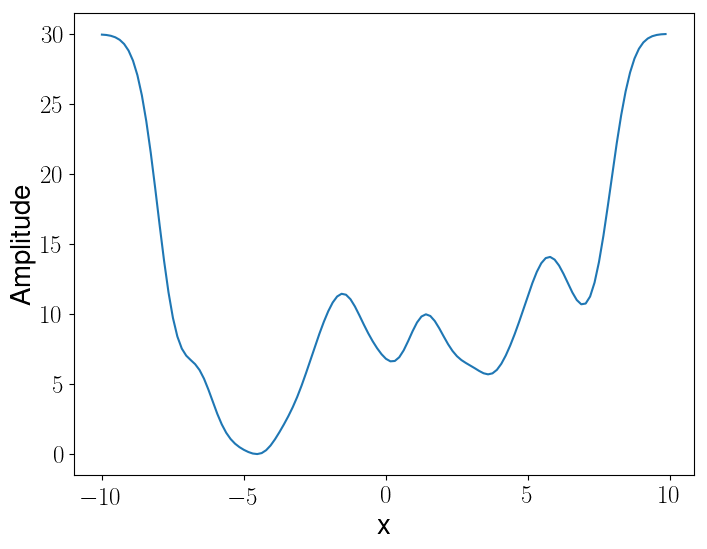
\includegraphics[width=\linewidth]{random-1-proc}
		
    \end{subfigure}
\caption{RandomPotential1 Before and After Process}
\label{fig:random1_before_after}
\end{figure}



The second one is summation of sines and cosines with random coefficients. Firstly, the number of terms are determined, after that each coefficient of the terms are assigned and summed iteratively.

\begin{algorithm}[H]
    \caption{RandomPotential2}\label{euclid}
    \begin{algorithmic}[1]
    \Procedure{RandomPotential2}{}
        \State $ Nterms = RandomInteger(1, 100)$
        \For{$\text{i} = 0 \textbf{ to } Nterms$}
        \State $A = GaussianDistributedRandomNumber()$
        \State $B = GaussianDistributedRandomNumber()$
        \State $n_1 = GaussianDistributedRandomNumber() * \sigma*\pi / width  $
        \State $n_2 = GaussianDistributedRandomNumber() * \sigma*\pi / width  $
        \State $Potential \mathrel{+}= A\sin(n_1 x) + B\cos(n_2 x)$
        \EndFor
        \State $Potential = GaussianFilter(Potential, \sigma)$ 
    \EndProcedure
    \end{algorithmic}
\label{alg:random_potential_1}
\end{algorithm}

\graphicspath{{"../figs/potentials/"}}
\begin{figure}[H]
    \centering
    \begin{subfigure}[t]{0.45\textwidth}
		%\centering
        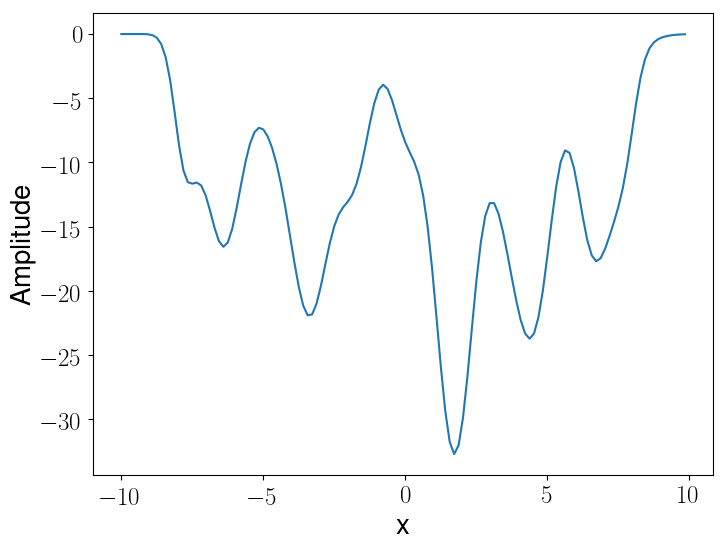
\includegraphics[width=\linewidth]{random-2-noproc}
		
    \end{subfigure}
    \begin{subfigure}[t]{0.45\textwidth}
		%\centering
        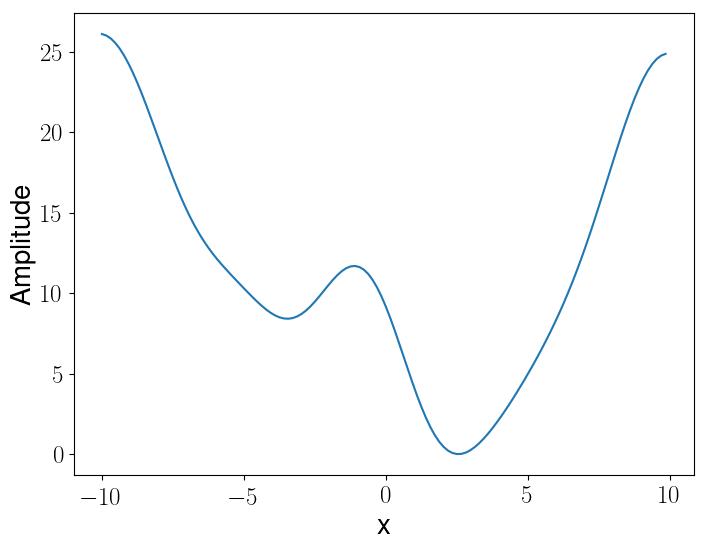
\includegraphics[width=\linewidth]{random-2-proc}
		
    \end{subfigure}
\caption{RandomPotential1 Before and After Process}
\label{fig:random2_before_after}
\end{figure}

The third one is one dimensional version of the algorithm described in \cite{mills2017deep} with slight modification. First a binary array of length $16$ is generated by assigning random ones or zeros. Then the array is upscaled to $128$ by repeating each element of the array $8$ times. After that, another binary array of length $8$ is generated with the same procedure and upscaled to $64$ by repeating elements. Left and right paddings of length $32$ is added to the second binary array to be able to do element wise substraction between two binary array. Then, the second array is substracted from the first one to obtain the potential in binary form. Finally, a gaussian filter is applied to make the potential smooth. 

\begin{algorithm}[H]
    \caption{RandomPotentia3}\label{euclid}
    \begin{algorithmic}[1]
    \Procedure{RandomPotential3}{}
        \State $ \textit{ScaleFactor} = 8$
        \For{$\text{i} = 0 \textbf{ to } \textit{NumberOfPoints/ScaleFactor}$}
        \State $BinaryGrid[i] = RandomInteger(0, 1)$
        \EndFor
        \State $BinaryGrid = RepeatElements(BinaryGrid, ScaleFactor)$
        \For{$\text{i} = 0 \textbf{ to } NumberOfPoints/(ScaleFactor * 2)$}
        \State $BinaryGrid2[i] = RandomInteger(0, 1)$
        \EndFor
        \State $BinaryGrid2 = RepeatElements(BinaryGrid, ScaleFactor)$
        \State $Padding = Zeros((Length(BinaryGrid) - Length(BinaryGrid2))/2)$
        \State $BinaryGrid2 = Concatanate(Padding, BinaryGrid2, Padding) $
        \State $Potential = BinaryGrid - BinaryGrid2$
        \State $Potential = GaussianFilter(Potential, \sigma)$ 
    \EndProcedure
    \end{algorithmic}
\label{alg:random_potential_1}
\end{algorithm}

\graphicspath{{"../figs/potentials/"}}
\begin{figure}[H]
    \centering
    \begin{subfigure}[t]{0.45\textwidth}
		%\centering
        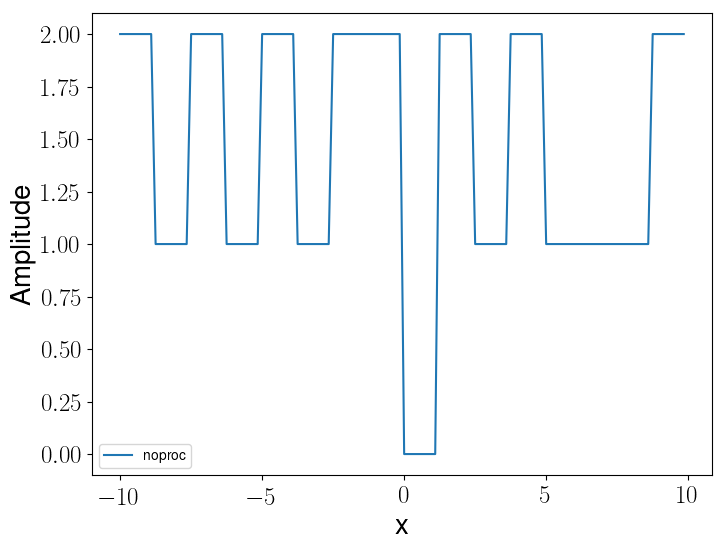
\includegraphics[width=\linewidth]{random-3-noproc}
		
    \end{subfigure}
    \begin{subfigure}[t]{0.45\textwidth}
		%\centering
        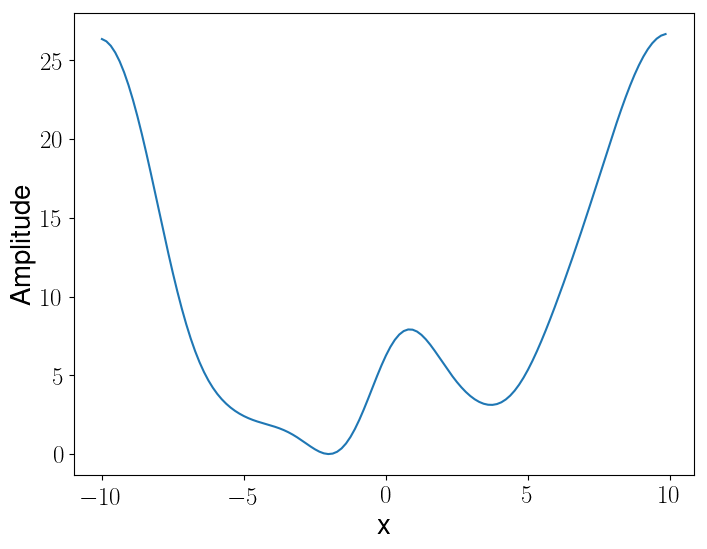
\includegraphics[width=\linewidth]{random-3-proc}
		
    \end{subfigure}
\caption{RandomPotential1 Before and After Process}
\label{fig:random3_before_after}
\end{figure}

\subsubsection{Density and Ground State Energy}

\graphicspath{{"../figs/potentials/"}}
\begin{figure}[H]
    \centering
    \begin{subfigure}[t]{0.45\textwidth}
        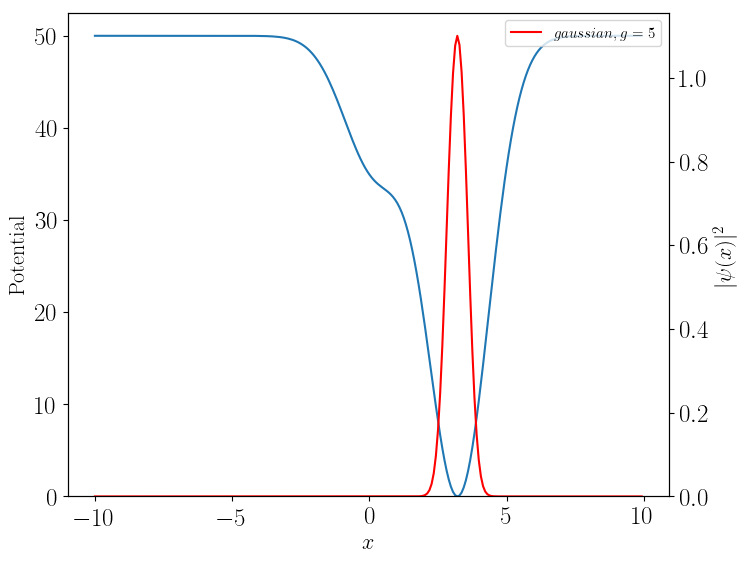
\includegraphics[width=\linewidth]{potvsdensity-gaussian}
    \end{subfigure}
    \begin{subfigure}[t]{0.45\textwidth}
        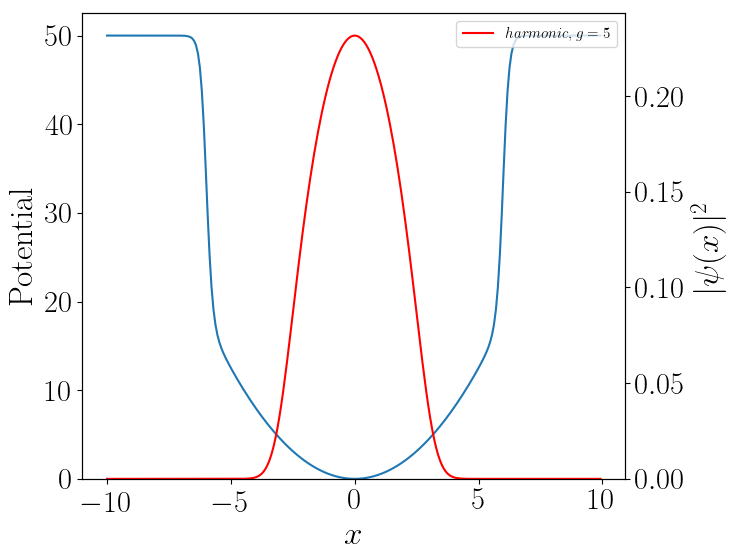
\includegraphics[width=\linewidth]{potvsdensity-harmonic}
    \end{subfigure}
    \begin{subfigure}[t]{0.45\textwidth}
        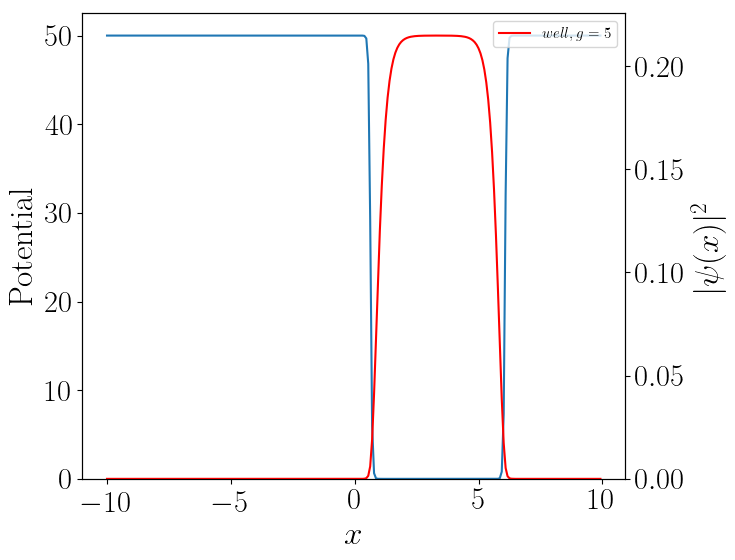
\includegraphics[width=\linewidth]{potvsdensity-well}
    \end{subfigure}
    \begin{subfigure}[t]{0.45\textwidth}
        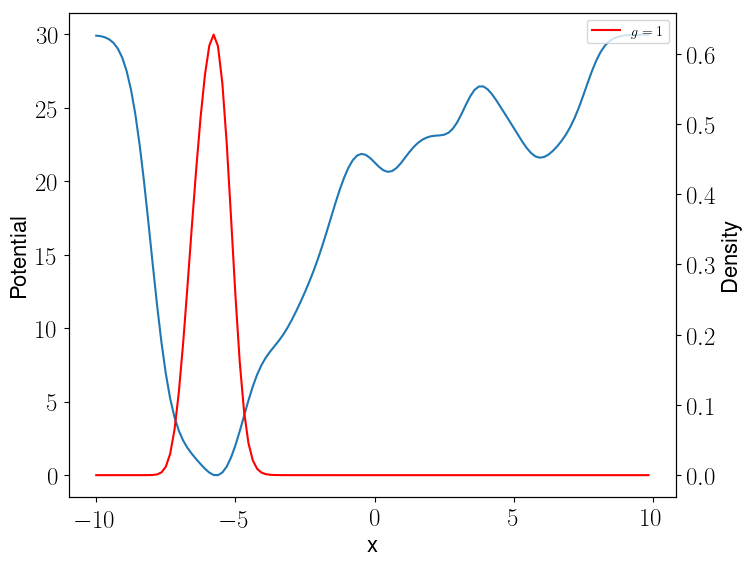
\includegraphics[width=\linewidth]{potvsdensity-random}
    \end{subfigure}
    \begin{subfigure}[t]{0.45\textwidth}
        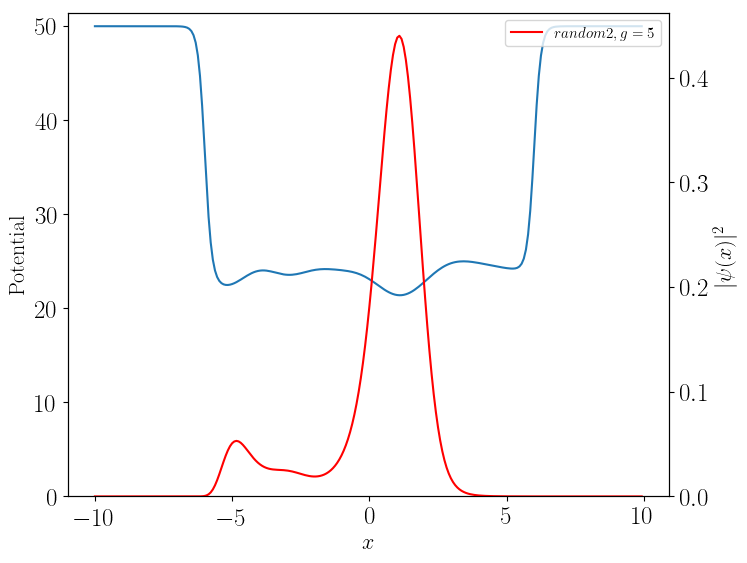
\includegraphics[width=\linewidth]{potvsdensity-random2}
    \end{subfigure}
    \begin{subfigure}[t]{0.45\textwidth}
        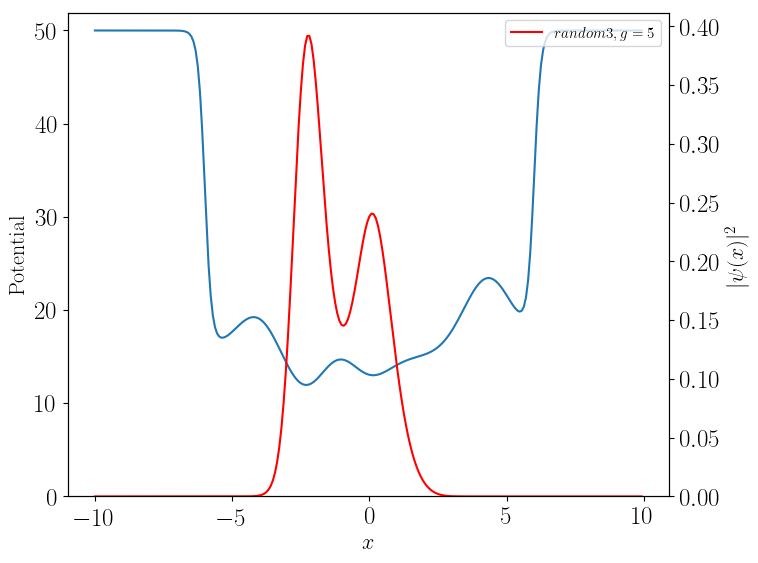
\includegraphics[width=\linewidth]{potvsdensity-random3}
    \end{subfigure}
\caption{RandomPotential1 Before and After Process}
\label{fig:random3_before_after}
\end{figure}





\subsubsection{Boundaries. (Table)}
\subsubsection{Convergence (detailed in APPENDIX)}
\subsubsection{Dataset generation. (Total number of examples etc)}

\subsection{Dataset Features}
\subsubsection{Energy distribution}

%\graphicspath{{"../figs/dataresults/gaussian/"}}
%\begin{figure}[H]
%    \centering
%    \begin{subfigure}[t]{0.45\textwidth}
%		%\centering
%        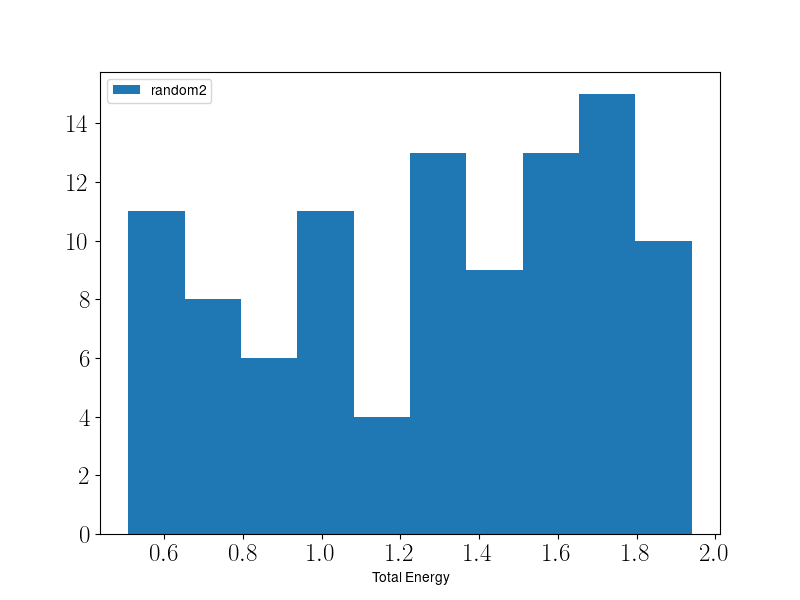
\includegraphics[width=\linewidth]{total}
%        \caption{g = 0}
%		
%    \end{subfigure}
%    \caption{Total energy distributions of the generated solution for different %interaction parameter values.}
%\label{fig:energy_dist}
%\end{figure}


\section{Machine Learning}
\subsection{Network architecture}
\noindent Architecture of the network.\\
    A general figure like in the ML\&SE article that describes the work done.\\
    Another figure about internals of the network such as number of layers, how interaction parameter is introduced to the network etc.\\
    Hyperparameters.\\
\subsection{Training}
\noindent    Detailed info about dataset (energy distribution etc).\\
    Indicate that if there is any method to increase the number of examples in low and high energy values.

\subsection{Results}

\section{Inverse Problem}

\clearpage
\section{Conclusion and Discussion}
\subsection{Conclusion}
\subsection{Discussion}
\subsection{Effects of random potential generation method}
\subsection{Are there problems in low and high energies compared to the mean}
\subsection{Inverse problem}


\clearpage

\clearpage
\bibliographystyle{ieeetr}
\bibliography{references}


\appendix
\section{APPENDIX A}
\label{ap:scale}

\textbf{Obtaining harmonic trap potential scaling from Eq.~\eqref{eq:GPE_dimensionless}}

\begin{equation}
\label{eq:GPESCALE_harmonic_potential_transform}
    V(z) \rightarrow V(\widetilde{z}) \rightarrow \widetilde{V}(\widetilde{z})
\end{equation}

\begin{equation}
\label{eq:GPESCALE_dimensionless_harmonic_potential}
    \widetilde{V}(z) \equiv \frac{V(z)}{\gamma E_0}
\end{equation}

\begin{equation}
\label{eq:GPESCALE_dimensionless_length}
    \widetilde{z} \equiv \frac{z}{\beta L} 
\end{equation}

\begin{equation}
\label{eq:GPESCALE_harmonic_potential}
    V(z) = \frac{1}{2}m\omega^2 (z-z_0)^2
\end{equation}

\begin{equation}
\label{eq:GPESCALE_harmonic_length_transform}
    V(\widetilde{z}) = \frac{1}{2}m\omega^2 \beta^2 L^2 (\widetilde{z}-\widetilde{z_0})^2
\end{equation}

\begin{equation}
\label{eq:GPESCALE_harmonic_energy_transform}
    \widetilde{V}(\widetilde{z}) = \frac{1}{2} m\omega^2 \frac{\beta^2 L^2}{\gamma E_0} (\widetilde{z}-\widetilde{z_0})^2  
\end{equation}

The coefficient of this equation must be dimensionless, therefore;

\begin{equation}
\label{eq:GPESCALE_harmonic_coeff}
    \frac{1}{2} m\omega^2 \frac{\beta^2 L^2}{\gamma E_0} = C
\end{equation}

Where $C$ is a positive constant. We know that $E_0 = \frac{\hbar^2}{2m}$ and the definition of $\alpha$ is given as,

\begin{equation}
\label{eq:GPESCALE_alpha}
    \frac{\hbar^2}{2m\gamma E_0} \frac{1}{\beta^2 L^2} = \alpha
\end{equation}
thus;

\begin{equation}
\label{eq:GPESCALE_gamma}
     \frac{1}{\gamma} = \alpha \beta^2 L^2
\end{equation}

if we plug Eq.~\eqref{eq:GPESCALE_gamma} in to Eq.~\eqref{eq:GPESCALE_harmonic_coeff}, then equation becomes,

\begin{equation}
\label{eq:GPESCALE_harmonic_coeff_2}
    \frac{m^2\omega^2}{\hbar^2} \alpha \beta^4 L^4 = C 
\end{equation} 

in the case of expressing same physical system, $m$ and $\omega$ must be constant. In that case $\alpha = C (\beta L)^{-4}$.\\


In this case, $\alpha$ becomes

$$ \alpha =  \frac{1}{2} \left(\frac{\hbar \omega}{\gamma E_0}\right)^2 $$

Conventionally, $\alpha$ is set to $1/2$, therefore;

$$ \hbar \omega = \gamma E_0 $$

$$ \beta L = \sqrt{\frac{\hbar}{m\omega}} $$ 

$ \beta L $ is generally defined as harmonic oscillator length $\ell$

$$ \ell = \sqrt{\frac{\hbar}{m\omega}} $$ 

$$ \widetilde{\mu} = \frac{\mu}{\hbar \omega} $$ 

$$ \widetilde{g} = \frac{g}{\hbar \omega \ell} $$

Finally, dimensionless GPE scaled for harmonic trapping potential can be written as,

$$\widetilde{\mu} \widetilde{\psi} = -\frac{1}{2}\frac{d^2\widetilde{\psi}}{d\widetilde{z}^2} + \frac{1}{2}\widetilde{z}^2\widetilde{\psi} + \widetilde{g}|\widetilde{\psi}|^2 \widetilde{\psi} $$


\end{document}
